\textbf{Why imitation instead of attacker?}

\subsection{Authentication Robustness of \systemname} After evaluating authentication accuracy for \systemname, we next study its robustness against imitation. For this purpose, we asked a number of subjects (imitators) to imitate simple nodding patterns from three subjects (imitatees) after watching the imitatee's video for as long as they desire, and calculated their chances of successful imitation - i.e., the imitator is mistakenly accepted by \systemname. We note that nodding is the simplest head-movement pattern and easiest to imitate; hence, the results presented here represent the \emph{lower bound} robustness that \systemname~offers. In reality, users are more likely to employ more sophisticated head-movement patterns, which will be much harder to imitate.

\subsubsection{Participants}
We had a total of 37 volunteer participants, including 31 males and 6 females. The average age of the participants was 25.6 years with a standard deviation
of 6.6 years. The youngest participant was 22 years old while the eldest was 49 years old.

\subsubsection{Procedure}
Our second experiment aimed at emulating a practical imitation attack scenario. In this experiment, three imitatees recorded video when they were nodding with a music cue. Note that the music is usually played via a bone conduction speaker or an earplug, and that it is difficult to use a camcorder to capture the music sound in a noisy environment. To address this concern, during recording, we set the speaker volume to maximum and conducted the recording in a quiet laboratory environment.

We divided the imitators into three group, and asked each group to imitated one imitatee. In each session (consisting of 30 trials), the imitator could watch the video for as long as they wish. Our system provided a feedback after each trial so that the imitators could adjust their nodding pattern if they wanted. After the imitator had 30 trials,
we ended the session no matter whether the imitator had succeeded or not. In each session, we noted the total number of successes the imitator had as well as the number of trail before the first successful imitation. %This experiment was conducted in quite space on campus. We will now discuss our evaluation results for both experiments in detail.

\subsubsection{Results}
Each of the three imitatees performed simple nodding in this experiment; though simple, their nodding patterns have varying complexity. As shown in Figure~\ref{fig:imitation_movement}, Imitatee $A$ moved his head vertically, each nodding on a music beat, with no noticeable horizontal movement; imitatee $B$ also only moved his head in the vertical direction, but there was always a delay between his nodding and the corresponding music beat; imitatee $C$ combined slight shaking along with nodding, and closely followed music beats. Among these three imitatees, $A$ is the easiest, while the other two are slightly more complex.

Table~\ref{tab:imitation} summarizes the results. Here, we use FAR to denote the successful imitation rate because a successful imitation is also a false acceptance. The overall FAR of the experiment is 7.54\%, while the individual FARs for the three imitatees are 15.83\%, 2.77\% and 2.72\% accordingly.  Since imitatee $A$ had the easiest nodding pattern, 6 out of 10 subjects could succeed at least once during their 30 trials, while for imitatees $B$ and $C$, the numbers are  3 out of 13 and 3 of 12, respectively. These results are promising: when a user employs slightly more complex head-movement patterns, it becomes much harder for others to imitate. 



\begin{table}[b]
\centering
\begin{tabular}{|l|c|c|c|c|}\hline
                               & No. &  No. &  Average No. of  &  \\
Imitatee & of & of & Trials Before & FAR (\%) \\
& Imitators & Successful Imitators & First Successful Login & \\\hline

A                   & 12                                 & 7                                                                     & 10.33                                                                                               & 15.83                        \\ \hline

B                   & 13                                 & 3                                                                     & 14.33                                                                                               & 2.77                         \\ \hline

C                   & 12                                 & 3                                                                     & 17.67                                                                                               & 2.72                          \\ \hline\hline

Overall & 38                                 & 13                                                                    & 13.17                                                                                                    & 6.94                         \\ \hline
\end{tabular}

\caption{\label{tab:imitation} The imitation results show that as head-movement patterns become more complex, it becomes much harder to imitate. }

\end{table}



\subsection{Headbanger Google Glass App Implementation}\label{subsec:app}

\begin{figure}[t]
\centering
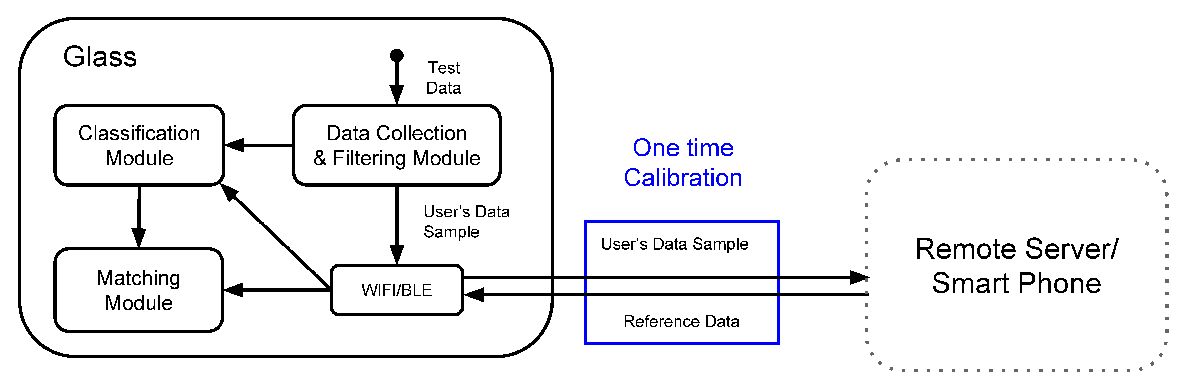
\includegraphics [width=\columnwidth]{figure/software_arch.eps}
\caption{Software modules of \systemname~implementation}
\vspace{25 pt}
\label{fig:glass-softwarearch}
\end{figure}

In the second phase of evaluation, we implemented \systemname~on Google glass
as an authentication app.
Figure~\ref{fig:glass-softwarearch} shows the main software modules in the
app. Upon initiation by the user, the app plays a music cue for a user-specified
duration. The user conducts head-movements in synchrony with the music cue
while the app records the accelerometer data in parallel. At the end of the
music cue duration the app enters the data processing phase where the
sensor readings are input to the \systemname's software modules for
processing. %The processing stage includes the filtering of the accelerometer
%sensor values, classification and feature extraction using DTW, and threshold
%based matching of the generated features with those from training set.
%%\systemname extracts the head-movement features through
%%the thresholding process discussed in section~\ref{sec:design}, and compare
%%with the feature templates generated from the training phase.
Upon completion of data processing, the app responds with a YES or NO textual
output on the Google Glass screen. The training phase is conducted offline on a PC, and %prior to live-testing off the application.
%The training phase 
%which involves collecting 30 samples of the
%head-movement accelerometer readings, generating the features, and saving them
%into a local server (running on PC) as an XML file, with appropriate indexing.
%Upon app initiation on Glass, the trained features are pre-fetched from
%the server through a wireless connection. 
we ensure that the training set
is readily available during the authentication process. %thus eliminating the
%additional processing time required for the training phase.
%Conducting online training, particularly that involves DTW computations, is
%very compute intensive on a resource constrained devices such as Glass.
%One possible solution would be for the Glass to offload the
%training phase computation to a local server machine.
%We reserve such considerations for future implementations.

%Among all the software modules, the ``training set construction model'' is
%the most computing-intensive, and as a result, we executed the model on the
%bluetooth-paired smartphone. The rest of the modules are implemented and
%executed on the glass.
%In our on-glass app, the classification module runs the
%thresholding-based classification.
\subsubsection{Data Processing Latency}

\begin{table}[b]
\centering
\begin{tabular}{|ccclc|}
\hline
\multicolumn{1}{|c|}{\multirow{2}{*}{\begin{tabular}[c]{@{}c@{}}music  cue \\
duration (s)\end{tabular}}} &
\multicolumn{1}{c|}{\multirow{2}{*}{\begin{tabular}[c]{@{}c@{}} data processing latency (s)\end{tabular}}} & \multicolumn{3}{c|}{time breakdown (\%)}
\\ \cline{3-5}
\multicolumn{1}{|c|}{}
                             &
\multicolumn{1}{c|}{}
                              &
 Filtering & \multicolumn{1}{c}{DTW} & Thresholding   \\
 \hline\hline
10
                             &
1.93
                              &
 0.50      & 99.50                   & \textless0.01  \\
6
                             &
1.15
                              &
 0.64      & 99.36                   & \textless0.01  \\
5
                             &
0.88
                              &
 0.81      & 99.19                   & \textless0.01 \\ \hline
\end{tabular}
\caption{\label{tab:glass} Measured response time of \systemname~app implementation on Google
Glass with different music cue durations and for $K = 1$. The response time
reported here is an average over 20 trials.}

\end{table}

In Table~\ref{tab:glass} we report the measured average processing latency
of the \systemname~app for music cue durations
of 5, 6 and 10 seconds. %We conducted the benchmark execution-time profiling of
%\systemname~on Glass in a controlled indoor laboratory setting with no
%mobility. We define response time as the time elapsed between music cue
%completion to
%the display of authentication response (YES/NO text) on the Glass screen.
The processing latency is within 2 seconds for a 10-second data input, and is less than 1 second (0.88s) for a 5-second input.  
%We feel that a response time of 2-5 sec for a local authentication solution in
%Google Glass is comparable to that of prior-art that comes close to our
%solution~\cite{von2013patterns,egelman2014you}.
%It is important to note that authentication solutions that execute
%locally on head-worn wearable devices, especially on a heavily resource
%constrained device like Glass, are still not mature. However, the hope is that
%such solutions will possibly catch up to speed in the near future and that our
%approach is advancing one step in that direction.
We also report the total latency breakdown for different software modules, and find that DTW computation is the main bottleneck. In our implementation, we used Fast DTW~\cite{salvador2007toward} which provides about 2x speed-up in DTW computation without compromising the authentication accuracy.
%We can observe from Table~\ref{tab:glass} that the DTW computation
%dramatically compute intensive than the other processes.

As we discussed earlier, the processing latency can be further reduced, and it could be partially hidden if we pipeline the data processing and data input. As a result, we believe that it is realistic to run the \systemname~app on devices that have comparable computing capabilities as the Google Glass.
%It is important to note that our current implementation uses a faster
%version of the DTW algorithm called Fast DTW~\cite{salvador2007toward},
%providing about 2x speed-up in DTW computation.
%We believe that the response time can be reduced
%further through strategic methods such as, further optimizations in the Fast
%DTW algorithm or pipelining the app execution along with data collection.
%A specific strategy for reducing response time for rejected attempts can be
%that, after a short duration, before the entire music cue is played, if it is
%found that a user's movement does not match the signature of the claimed user
%with a sufficient pre-determined confidence level, then the on-site
%classification may be terminated instead of waiting for the entire duration to
%yield the rejection.
%Another example, may include cyber-foraging strategies to offload heavy
%computation tasks, such as online training and classification, to the user's
%Bluetooth paired smartphone or a nearby cloudlet~\cite{ha2014towards}.

